

\subsection{Control system}
\label{sec:control_system}

For controlling the motor, the output d- and q-current of the motor are feedback to a PI-controller for each of them. The d-current is desired to be zero, and is therefore compared with zero before the PI-controller. The q-current is desired to be set to the reference point set by the input from the torque pedal. The torque reference input is therefore converted to a current, which can be compared with the feedback q-current from the motor model.

After the PI-controller the d- and q-voltages are converted back into three phases with an Inverse Clarke and an Inverse Park transformation. The three phase voltages are then put into the motor model.

The full model of the system can be seen on figure \ref{fig:control_system}.


\begin{figure}[H]
	\centering
	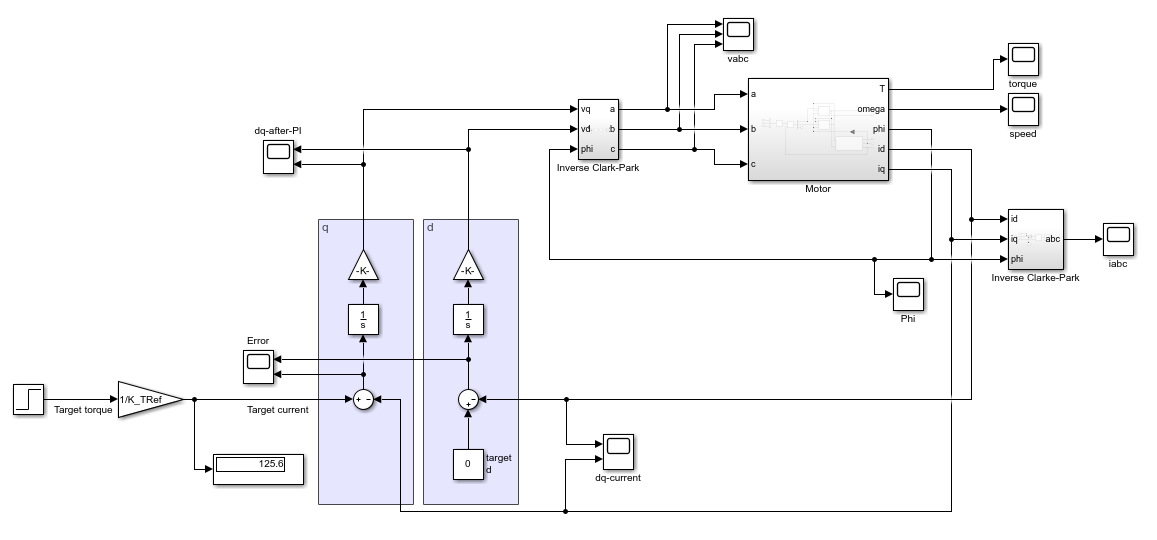
\includegraphics[width=1\linewidth]{pictures/control/full_model.PNG}
	\caption{The entire control model, with PI controller and motor model.}
	\label{fig:control_system}
\end{figure}

